\documentclass[10pt,a4paper]{article}

\usepackage[title=true,titlestyle=small]{../phfnote}
%\usepackage{../phfnote}
\def\mypkgs{
  \usepackage{amsmath}
  \usepackage{amsfonts}
  \usepackage{amsthm}
  \usepackage{xcolor}
  \usepackage[shortlabels]{enumitem}
  \theoremstyle{plain}
  \newtheorem{thm}{Theorem}
  \newtheorem{prop}[thm]{Proposition}
  \newtheorem{lemma}[thm]{Lemma}
  \newtheorem{cor}[thm]{Corollary}
  \newtheorem{conj}[thm]{Conjecture}
  \newtheorem{remark}[thm]{Remark}
  \newtheorem*{thm*}{Theorem}
  \newtheorem*{prop*}{Proposition}
  \newtheorem*{lemma*}{Lemma}
  \newtheorem*{cor*}{Corollary}
  \newtheorem*{conj*}{Conjecture}
  \newtheorem*{idea*}{Idea}
  \newtheorem*{remark*}{Remark}
}
%\mypkgs


\def\noteabstracttextfont{\small\itshape}


\usepackage{../phfqit}


% fully mixed state, \Ident_X/|X|
\newcommand{\Mixed}[1]{{\frac{\Ident_{#1}}{\abs{#1}}}}
% fully mixed state, \Ident_X/|X|, text-style fraction
\newcommand{\Mixedi}[1]{{\textstyle\frac{\Ident_{#1}}{\abs{#1}}}}
% fully mixed state, \Ident_n/n
\newcommand{\Mixedn}[1]{{\frac{\Ident_{#1}}{#1}}}
% fully mixed state, \Ident_n/n, text-style fraction
\newcommand{\Mixedin}[1]{{\textstyle\frac{\Ident_{#1}}{#1}}}


% hilbert spaces & entropies & spaces...
\def\Hs{\mathscr{H}}% Hilbert space
\def\Hamilt{\mathcal{H}}% Hamiltonian
\def\HH{{H}}% Entropy-denoting 'H' letter
\def\Hmin{\HH_\mathrm{min}}
\def\Hmax{\HH_\mathrm{max}}
\def\Hzero{\HH_0}



% custom style for proofs
\definecolor{prooftextcolor}{rgb}{0.,0.,0.}
\newenvironment{myproof}[1][\proofname]{%
  \color{prooftextcolor} \footnotesize \proof[\itshape #1]\hspace*{1.2mm}%
}{\endproof}


%\usepackage{txfonts}
%\usepackage{multicol}


\newcommand{\lD}{\lambda^\downarrow}
\newcommand{\lU}{\lambda^\uparrow}
\newcommand{\lambdamaj}[1]{\xrightarrow{#1}}
\newcommand{\LOps}{\mathscr{L}}
\newcommand{\POps}{\mathscr{P}}
\newcommand{\DOps}{\mathscr{S}_=}

\title{Notes on Lambda-Majorization}
\author{Ph. F.}
\date{\today}

\begin{document}
\maketitle
%\setlength{\noteabstracttextwidth}{\textwidth}
%\setlength{\noteabstractafterspacing}{0mm}
%\renewcommand{\noteabstracttextfont}{}

\begin{abstract}
  We characterize the work cost of state transitions using a framework based on Landauer's Principle and
  on the so-called noisy operations introduced by~[Horodecki et al, PRA, 2003]. Noisy operations correspond to
  adding a fully mixed ancilla, performing a unitary, and removing the ancilla. Previous work has demonstrated
  the relation between these operations and the mathematical notion of majorization. Using Landauer's Principle,
  we reduce the characterization of work cost or extraction to the consideration of absorbtion or generation
  during noisy operations of randomness stored in ancillas, similar to the notion of thermomajorization introduced
  by Horodecki et al.~[arXiv:1111.3834v1]. This framework provides a
  suitable tool to find a lower bound to the work cost of the erasure of a system possessing quantum
  correlations with a memory, expressed as the min-entropy of the system conditioned on the memory. This
  bound is complementary to the upper bound presented in~[del Rio et al., Nature, 2011].
\end{abstract}


\inlinetoc

\section{Introduction and Framework}

This example document contains early material which was ultimately further developed and
published open-access in \emph{Nature Communications},
\url{http://dx.doi.org/10.1038/ncomms8669}.

\begin{figure}[t]
  \centering
  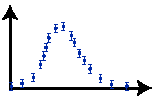
\includegraphics[width=3cm]{testfigure}
  \caption{Test figure. This should not appear at the top where the title is.}
  \label{fig:test}
\end{figure}

Landauer's Principle~\cite{Landauer1961_5392446Erasure}, and more generally the relation between the second law
of thermodynamics and information theory, has driven much attention in the past decades. Studies have notably
focused on heat generated by computation~\cite{Bennett1982IJTP_ThermodynOfComp}, the exorcism of Maxwell's demon
via information theory (see eg.~\cite{Bennett2003_NotesLP}), and generalizations to quantum settings such as
characterization of entanglement through thermodynamical
considerations~\cite{Oppenheim2002PRL_thermodynamical}, or the determination of the single shot work cost of
the erasure of a quantum system with quantum side information~\cite{delRio2011Nature}.

Some previous work has attempted to justify Landauer's Principle and generalizations
through explicit models such as Szilard
boxes~\cite{Szilard1929ZeitschriftFuerPhysik,Dahlsten2011NJP_inadequacy}, or explicit
Hamiltonian models~\cite{Alicki2004_hamiltonian}, all of which are NOT depicted in
\figurename~\ref{fig:test}. We will follow a different approach by assuming Landauer's
Principle as being valid, much like one generally accepts the second law of thermodynamics
as being valid. This allows us to {\em define} a notion of work in our quantum setting by
characterizing how much randomness can be absorbed or is generated during a noisy
operation.

This notion is closely related to the notion of {\em themomajorization} introduced by
Horodecki et al.~\cite{Horodecki2013_ThermoMaj}. However, while their approach is to model
the thermodynamics of physical systems with more realistic non-degenerate Hamiltonians, we
adopt in contrast a purely information-theoretical point of view with degenerate
Hamiltonians and unitary computations.

Consider a quantum mechanical system $X$ in an inital state described by the density operator $\sigma$.
Our task is to bring the system $X$ to another state $\rho$, while attempting to maximize some kind of notion
of ``extracted'' work in the process.

The allowed operations are:
\begin{enumerate}[(a)]
\item Bring the system $X$ (or an ancilla $A$) of $n$ qubits from any state to a pure state (`erasure') at
  cost $n\,kT\ln 2$ work;
\item Bring the system $X$ (or an ancilla $A$) of $n$ qubits from a pure state to a fully mixed state while
  extracting $n\,kT\ln 2$ work;
\item Add and remove ancillas in pure or fully mixed states at no work cost, as long as all the ancillas have
  been restored to their initial state at the end of the process;
\item Perform arbitrary unitaries (over $S$ and any added ancillas) at no work cost.
\end{enumerate}

\subsection{Test Subsection}

Note that operations (a) and (b) are merely a statement of Landauer's Principle. These operations
may be carried out for example with a Hamiltionian description as presented in~\cite{delRio2011Nature}.
Operations (a) and (b) define a quantity that we call in this context ``work''.

This \rule{5em}{1ex} \rule{5em}{1ex} paragraph \rule{5em}{1ex} might \rule{5em}{1ex} have
\rule{5em}{1ex} long \rule{5em}{1ex} words \rule{5em}{1ex} which \rule{5em}{1ex} can't
\rule{5em}{1ex} be \rule{5em}{1ex} broken.
%
And this \rule{15em}{1ex} \rule{15em}{1ex} paragraph \rule{15em}{1ex} might
\rule{15em}{1ex} have \rule{15em}{1ex} long \rule{15em}{1ex} words \rule{15em}{1ex} which
\rule{15em}{1ex} can't \rule{15em}{1ex} be \rule{15em}{1ex} broken.

\subsection{Test Another Subsection}

On the other hand, operations (c) and (d) are purely information-theoretical. We assume here that the Hamiltonian
of the system is completely degenerate. These operations allow the use of noisy operations, which correspond to
adding an ancilla $Y$ in a fully mixed state, performing a unitary, and removing the ancilla. Previous work by
Horodecki et al.~\cite{Horodecki2003PRA_NoisyOps} has shown the following important relation between noisy
operations and the mathematical notion of
majorization~\cite{BookBhatiaMatrixAnalysis1997,BookHornJohnsonMatrixAnalysis1985}.

\paragraph{Noisy Operations and Majorization.}
The transition on system $X$ from state $\sigma$ to state $\rho$ is possible by noisy operation if and
only if $\sigma\succ\rho$.


\section{Lambda-Majorization: Definition, Characterization and Properties}

\subsection{Overview}
We will characterize our randomness absorption process in terms of a gerenalized notion of doubly
substochastic matrices.

Recall that majorization between two normalized states is exactly characterized by the existance of
a doubly substochastic matrix relating both spectra~\cite{BookBhatiaMatrixAnalysis1997}. A doubly
substochastic matrix $S_i^{~j}$ satisfies
$S_i^{~j}\geqslant 0$, $\sum_i S_i^{~j} \leqslant 1$, $\sum_j S_i^{~j} \leqslant 1$.
\begin{prop}
  \label{prop:majorizationDoublyStochMatrix}
  Two (normalized) density matrices $\sigma$ and $\rho$ satisfy $\sigma\succ\rho$ if and only if
  there exists a doubly substochastic matrix $S_i^{~j}$ such that
  $\lambda_i(\rho) = \sum_j S_i^{~j}\lambda_j(\sigma)$ .
\end{prop}

Majorization defines a {\em partial order} on states and has a ``smallest'' element, the fully mixed state. Also,
a pure state majorizes any other state.

Majorization is preserved by direct sums and tensor products, i.e. if $v\succ w$ and $v'\succ w'$, then
$v\oplus v' \succ w\oplus w'$ and $v\otimes v' \succ w\otimes w'$.

\paragraph{Lambda-Majorization.} We will write $\sigma\lambdamaj{\lambda}\rho$ if there exists
$\lambda_1,\lambda_2\geqslant 0$, with $\lambda=\lambda_1-\lambda_2,$ such
that $2^{-\lambda_1}\Ident_{2^{\lambda_1}}\otimes\sigma \succ 2^{-\lambda_2}\Ident_{2^{\lambda_2}}\otimes\rho$.

The link to extractable work can be seen if we have to restore ancillas to their original state. If during
the noisy operation process an ancilla was brought from a fully mixed state to a pure state, operation (b)
allows us to extract work. Conversely, work is paid if an originally pure ancilla was left in a mixed
state.

Our generalization of Proposition~\ref{prop:majorizationDoublyStochMatrix} says that the notion of
randomness absorption in a majorization can be captured in
the way the doubly substochastic map is normalized.
\begin{prop}
  \label{prop:LambdaMajTik}
  Two (normalized) density matrices $\sigma$ and $\rho$ satisfy $\sigma\lambdamaj{\lambda}\rho$
  if and only if there exists a matrix $T_i^{~k}$ such that $\lambda_i(\rho) = \sum_k T_i^{~k}\lambda_k(\sigma)$,
  where $T_i^{~k}\geqslant 0$, $\sum_i T_i^{~k} \leqslant 1$ and $\sum_k T_i^{~k} \leqslant 2^{-\lambda}$ .
\end{prop}

Note that by using the generalized substochastic maps (instead of stochastic maps), one can cut out the parts
of the matrix that deal with the zero eigenvalues of $\rho$ and $\sigma$ (a submatrix of a doubly substochastic
matrix is itself doubly substochastic). Thus without loss of generality one can look at the vectors of
non-zero eigenvalues of $\rho$ and $\sigma$, and the dimensions of the systems in which they are embedded are
irrelevant.

Note also that density matrices are understood to be {\em normalized}, i.e. $\tr\sigma=\tr\rho=1$. Subnormalized
states will be denoted as such and not be called density matrices. Considering normalized states allows to
directly imply a full majorization from a weak majorization, since the equality condition is automatically
satisfied.


\subsection{Formal Definitions and Properties}

Let $\Hs_X$, $\Hs_Y$ be two subspaces of a large (finite) Hilbert space $\Hs_Z$, and let
$\Hs_A$, $\Hs_B$ be two subspaces of a (finite-dimensional) Hilbert space $\Hs_C$. Let $d_{(\cdot)}$ denote
 the dimensions of the various Hilbert
spaces $\Hs_{(\cdot)}$ and specifically let $d=d_Z=\dim\Hs_Z$. Denote by $\LOps(\Hs)$ the set of linear
hermitian operators on $\Hs$, by $\POps(\Hs)$ the set of positive semidefinite operators on $\Hs$, and
by $\DOps(\Hs)$ those operators in $\LOps(\Hs)$ that have unit trace.

\paragraph{Majorization.} A matrix $\sigma\in\POps(\Hs_Z)$ is said to {\em majorize} $\rho\in\POps(\Hs_Z)$
(denoted by $\sigma\succ\rho$) if for all $k$, $\sum_{i=1}^k \lD_i(\sigma) \geqslant \sum_{i=1}^k \lD_i(\rho)$,
and if $\tr\sigma=\tr\rho$.

The notion of majorization defines a (partial) order relation on $\POps(\Hs_Z)$. When looking at the
set of density matrices $\DOps(\Hs_Z)$, there is a ``least'' element: the fully mixed state,
$\frac{1}{d}\Ident_Z$.

\paragraph{Weak Submajorization.} A matrix $\sigma\in\POps(\Hs_Z)$ is said to {\em weakly submajorize}
$\rho\in\POps(\Hs_Z)$ (denoted by $\sigma\succ_w\rho$) if for all $k$,
$\sum_{i=1}^k \lD_i(\sigma) \geqslant \sum_{i=1}^k \lD_i(\rho)$.

\begin{remark*}
  If $\sigma,\rho\in\DOps(\Hs_Z)$, then the concept of weak submajorization is equivalent to (full)
  majorization because the matrices are automatically normalized.
\end{remark*}

\paragraph{Doubly Stochastic Matrix.} A $d\times d$ matrix $S$ is {\em doubly stochastic} if
$S_i^{~j}\geqslant 0$, $\sum_i S_i^{~j} = 1~\forall\,j$ and $\sum_j S_i^{~j} = 1~\forall\,i$.

\paragraph{Doubly Substochastic Matrix.} A $n\times m$ matrix $B$ is {\em doubly substochastic} if
$B_i^{~j}\geqslant 0$, $\sum_i B_i^{~j} \leqslant 1~\forall\,j$ and $\sum_j B_i^{~j} \leqslant 1~\forall\,i$.

The following proposition is due to Hardy, Littlewood and P\'olya~\cite{HardyLittlewoodPolyaInequalities1952}.

\begin{prop}[Hardy, Littlewood, and P\'olya, 1929]
  \label{prop:MajDblStochEquiv}
  Let $\sigma,\rho \in \POps(\Hs_Z)$. Then $\sigma\succ\rho$ if and only if there exists a $d\times d$
  doubly stochastic matrix $S_i^{~j}$ such that $\lambda_i(\rho) = \sum_j S_i^{~j}\lambda_j(\sigma)$ .
\end{prop}

\begin{prop}
  \label{prop:WeakMajDblSubstochEquiv}
  Let $\sigma \in \POps(\Hs_X)$ and $\rho\in\POps(\Hs_Y)$. Then $\sigma\succ_w\rho$ if and only if there
  exists a $d_Y \times d_X$ doubly substochastic matrix $B_i^{~j}$ such that
  $\lambda_i(\rho) = \sum_j B_i^{~j}\lambda_j(\sigma)$ .
\end{prop}


Now we will define the concept of {\em Lambda-Majorization}, or {\em Majorization with Randomness Absorption}.
The idea is to characterize ``how well'' a state $\sigma$ majorizes a state $\rho$. If a state $\sigma$ majorizes
$\rho$, then maybe there is some margin for absorbing some randomness, say, maybe the state
$\frac12\Ident_2\otimes\sigma$ still majorizes $\rho$. This corresponds to erasing a fully mixed qubit at the same time
as performing the transition from $\sigma$ to $\rho$. On the other hand, if $\sigma$
does not majorize $\rho$, it will however majorize the state $\frac1n\Ident_n\otimes\rho$ for some $n$ big enough.

For a formal definition, let $\lambda\in\mathbb{R}$ and let $\lambda_1,\lambda_2\geqslant 0$ such that
$\lambda = \lambda_1-\lambda_2$ and $2^{\lambda_1}$,$2^{\lambda_2}$ are integers\footnote{in case $2^\lambda$ is
  irrational, approximate $2^\lambda$ arbitrarily well by a rational number $2^{\lambda'}$, and the definition
  will have to be satisfied for arbitrarily good such rational approximations.}.
Take $\Hs_C$ of size greater than both $2^{\lambda_1}$ and $2^{\lambda_2}$ and let $\Hs_A$ and $\Hs_B$ be subspaces
of $\Hs_C$ of respective dimensions $2^{\lambda_1}$ and $2^{\lambda_2}$.

\paragraph{Lambda-Majorization.} We say that $\sigma\in\POps(\Hs_X)$ {\em $\lambda$-majorizes}
$\rho\in\POps(\Hs_Y)$ (denoted by $\sigma\lambdamaj\lambda\rho$) if there exists such
$\lambda_1$, $\lambda_2$ such that
$2^{-\lambda_1}\Ident_A\otimes\sigma \succ_w 2^{-\lambda_2}\Ident_B\otimes\rho$.
Here $\Ident_A$, $\Ident_B$ are the projectors onto the respective subspaces $\Hs_A$ and $\Hs_B$
embedded in $\Hs_C$. Likewise, $\sigma$ and $\rho$ are considered as living in $\Hs_Z$ (pad them with zero
eigenvalues).

\begin{prop}
  \label{prop:LambdaMajMoveIdentitiesAround}
  For any $\sigma\in\POps(\Hs_X)$, $\rho\in\POps(\Hs_Y)$, and for any $\lambda\in\mathbb{R}$, $n\geqslant 0$, we have
  \begin{align*}
    {\textstyle\frac1n}\Ident_n\otimes\sigma\lambdamaj\lambda\rho  ~\Leftrightarrow~
    \sigma\lambdamaj{\lambda+\log n} \rho
  \end{align*}
  and
  \begin{align*}
    \sigma\lambdamaj{\lambda-\log n} \rho  ~\Leftrightarrow~
    \sigma\lambdamaj\lambda {\textstyle\frac1n}\Ident_n\otimes\rho\ .
  \end{align*}
\end{prop}

\begin{prop}[General version of Prop.~\ref{prop:LambdaMajTik}]
  \label{prop:LambdaMajTikFormal}
  Let $\sigma\in\POps(\Hs_X)$ and $\rho\in\POps(\Hs_Y)$. Then $\sigma\lambdamaj\lambda\rho$ if
  and only if there exists a $d_Y \times d_X$ matrix $T_i^{~k}$ such that
  $\lambda_i(\rho) = \sum_k T_i^{~k} \lambda_k(\sigma)$, and that satisfies
  $T_i^{~k}\geqslant 0$,
  $\sum_i T_i^{~k} \leqslant 1$, and
  $\sum_k T_i^{~k} \leqslant 2^{-\lambda}$ .
\end{prop}

\begin{myproof}[Proof of Prop.~\ref{prop:LambdaMajTikFormal}]
  Suppose $2^{-\lambda_1}\Ident_A\otimes\sigma\succ_w 2^{-\lambda_2}\Ident_B\otimes\rho$
  with $\lambda=\lambda_1-\lambda_2$. Then there exists a doubly substochastic matrix $S_{bi}^{~ak}$ such that
  \begin{align*}
    \lambda_{bi}\bigl(2^{-\lambda_2}\Ident_B\otimes\rho\bigr)
    = \sum_{ak} S_{bi}^{~ak}\, \lambda_{ak}\bigl( 2^{-\lambda_1}\Ident_A\otimes\sigma\bigr)\ ,
  \end{align*}
  with $S_{bi}^{~ak}\geqslant 0$, $\sum_{bi} S_{bi}^{~ak} \leqslant 1$ and $\sum_{ak} S_{bi}^{~ak}\leqslant 1$.
  (Indices $a$ and $b$ refer to the mixed ancillas of respective sizes $2^{\lambda_1}$ and $2^{\lambda_2}$.)

  Now we have
  \begin{align*}
    \lambda_i\bigl(\rho\bigr) &= \sum_b \lambda_{bi}\bigl(2^{-\lambda_2}\Ident_B\otimes\rho\bigr) \\
    &= \sum_{a\,b\,k} S_{bi}^{~ak}\,\lambda_{ak}\bigl(2^{-\lambda_1}\Ident_A\otimes\sigma\bigr) \\
    &= \sum_k \left(\sum_{ab}2^{-\lambda_1}\,S_{bi}^{~ak}\right)\,\lambda_k\left(\sigma\right)\ ,
  \end{align*}
  so one can define
  \begin{align*}
    T_i^{~k} = \sum_{ab} 2^{-\lambda_1}\,S_{bi}^{~ak}\ ,
  \end{align*}
  which fulfills $\lambda_i\bigl(\rho\bigr) = \sum_k T_i^{~k}\,\lambda_k\bigl(\sigma\bigr)$. Because $S$ is
  doubly substochastic, and using the fact that indices $a$ (resp. $b$) range to $2^{\lambda_1}$
  ($2^{\lambda_2}$), the matrix $T$ satisfies
  \begin{align*}
    \sum_i T_i^{~k} = \sum_{i\,a\,b} 2^{-\lambda_1} S_{bi}^{~ak}
    = \sum_a 2^{-\lambda_1}\sum_{bi} S_{bi}^{~ak} \leqslant 1\ ,
  \end{align*}
  as well as
  \begin{multline*}
    \sum_k T_i^{~k} = \sum_{k\,a\,b} 2^{-\lambda_1}S_{bi}^{~ak} \\
    = \sum_b 2^{-\lambda_1}\,\sum_{ak}S_{bi}^{~ak} \leqslant \sum_b 2^{-\lambda_1} = 2^{-\lambda}\ .
  \end{multline*}
  Additionally, $T_i^{~k}\geqslant 0$ because $S_{bi}^{~ak}\geqslant 0$.

  Conversely, suppose that a matrix $T_i^{~k}$ exists, with $T_i^{~k}\geqslant 0$,
  $\sum_i T_i^{~k} \leqslant 1$, $\sum_k T_i^{~k} \leqslant 2^{-\lambda}$, and
  $\lambda_i(\rho) = \sum_k T_i^{~k} \lambda_k(\sigma)$. Let $\lambda_1,\lambda_2$ such that
  $\lambda=\lambda_1-\lambda_2$ and such that $2^{\lambda_1}$, $2^{\lambda_2}$ are integers.
  Then let $S_{bi}^{~ak} = 2^{-\lambda_2}T_i^{~k}$ for all $a$, $b$. Then $S_{bi}^{~ak} \geqslant 0$ and
  $S$ satisfies
  \begin{multline*}
    \sum_{ak} S_{bi}^{~ak} = 2^{-\lambda_2}\sum_{ak}T_i^{~k} 
    \leqslant 2^{-\lambda_2} \Bigl(\sum_a 1\Bigr)\; 2^{-\lambda} = 1\ ,
  \end{multline*}
  as well as
  \begin{multline*}
    \sum_{bi} S_{bi}^{~ak} = 2^{-\lambda_2} \sum_{bi} T_i^{~k} 
    \leqslant 2^{-\lambda_2}\Bigl(\sum_b 1\Bigr) = 1\ .
  \end{multline*}
  The required lambda-majorization is provided by this doubly substochastic matrix,
  \begin{multline}
    \hspace*{-4mm}\lambda_{bi}\bigl(2^{-\lambda_2}\Ident_B\otimes\rho\bigr)
    = 2^{-\lambda_2}\lambda_i\bigl(\rho\bigr)
    = 2^{-\lambda_2} \sum_k T_i^{~k} \lambda_k\bigl(\sigma\bigr) \\
    = 2^{-\lambda_2} \sum_k T_i^{~k} \sum_a\lambda_{ak}\bigl(2^{-\lambda_1}\Ident_A\otimes\sigma\bigr)\\
    = \sum_{ak} S_{bi}^{~ak}\lambda_{ak}\bigl(2^{-\lambda_1}\Ident_A\otimes\sigma\bigr)\ .\tag*{\qedhere}
  \end{multline}
\end{myproof}


\subsection{Properties in case of normalized states}

Some useful properties of lambda-majorization in the case we consider normalized states $\sigma$, $\rho$. In
this case, weak majorization automatically implies (full) majorization because $\tr\sigma=\tr\rho=1$.

In this section, let $\sigma\in\DOps(\Hs_X)$ and $\rho\in\DOps(\Hs_Y)$.

\begin{prop}[Lambda-Majorizing a Pure State]
  \label{prop:lambdaMajDOpsPureState}
  For any pure state $\ket 0\in\Hs_Z$, we have $\sigma\lambdamaj\lambda\ketbra00$ if and only
  if $\rank\sigma\leqslant 2^{-\lambda}$.
  Equivalently, $\sigma\succ\frac1n\Ident_n$ if and only if $\rank\sigma\leqslant n$.
\end{prop}

\begin{myproof}[Proof of Prop.~\ref{prop:lambdaMajDOpsPureState}]
  Assume first that  $\sigma\lambdamaj\lambda\ketbra00$. Here $\Hs_Y$ is the one-dimensional space
  spanned by $\ket0$, and take $\Hs_X$ the subspace on which $\sigma$ has its support. By
  Prop.~\ref{prop:LambdaMajTikFormal} there exists a single-row matrix
  $T_i^{~k}$ satisfying $T_i^{~k}\geqslant 0$, $\sum_i T_i^{~k} = T_{i=1}^{~k} \leqslant 1~\forall k$,
  $\sum_k T_i^{~k} \leqslant 2^{-\lambda}$ such that
  $1 = \lambda_{i=1}(\ketbra00) = \sum_k T_{i=1}^{~k} \lambda_k(\sigma)$. We also have $\lambda_k(\sigma)\neq 0$
  because $\sigma$ has nonzero eigenvalues in $\Hs_X$. Then
  $\sum_k T_{i=1}^{~k} \lambda_k(\sigma) = 1 = \sum_k\lambda_k(\sigma)$ implies $T_{i=1}^k = 1~\forall k$.
  That is, the condition $\sum_k T_{i=1}^{~k} \leqslant 2^{-\lambda}$ forces $T_{i=1}^{~k}$ to have at most
  $2^{-\lambda}$ elements, i.e. the rank of $\sigma$ may not exceed $2^{-\lambda}=2^{-\lambda} \rank\rho$.

  The converse holds because any state majorizes a uniform state of same rank.
\end{myproof}

\begin{prop}[Condition on Support Sizes for Lambda-Majorization]
  \label{prop:lambdaMajDOpsConditionRanks}
  If $\sigma\lambdamaj\lambda\rho$, then $\rank\sigma\leqslant 2^{-\lambda}\rank\rho$. 
\end{prop}

\begin{myproof}[Proof of Prop.~\ref{prop:lambdaMajDOpsConditionRanks}]
  Notice that $\rho\succ\frac1{\rank\rho}\Ident_{\rank\rho}$, thus
  $\sigma\lambdamaj\lambda\frac1{\rank\rho}\Ident_{\rank\rho}$, and by
  Prop.~\ref{prop:LambdaMajMoveIdentitiesAround},
  \begin{equation*}
    \sigma\lambdamaj{\lambda-\log\rank\rho} \ketbra00\ ;
  \end{equation*}
  it remains to apply Prop.~\ref{prop:lambdaMajDOpsPureState}.
\end{myproof}


\begin{prop}[Being Lambda-Majorized by a Pure State]
  \label{prop:LambdaMajorizedDOpsByPureState}
  Let the state $\rho$ have maximum eigenvalue $\lambda_\mathrm{max}(\rho)$.
  For any pure state $\ket0$, we have $\ketbra00 \lambdamaj\lambda \rho$ if and only if
  $\lambda_\mathrm{max}(\rho) \leqslant 2^{-\lambda}$. Equivalently, $\frac1n\Ident_n\succ\rho$ if and
  only if $\lambda_\mathrm{max}(\rho) \leqslant \frac1n$.
\end{prop}

\begin{myproof}[Proof of Prop.~\ref{prop:LambdaMajorizedDOpsByPureState}]
  Let $T_i^{~k}$ be such as in Prop.~\ref{prop:LambdaMajTikFormal}. Note here $k$ only takes value
  $1$, because we consider $\Hs_Y$ being the one-dimensional space spannded by $\ket0$. Then
  $\lambda_i(\rho) = \sum_k T_i^{~k} \lambda_k(\ketbra00) = T_i^{~k=1}$ and thus
  $T_i^{~k}=\lambda_i(\rho)$. Then $2^{-\lambda} \geqslant \sum_k T_i^{~k} = T_i^{k=1} = \lambda_i(\rho)$ for
  all $i$. In particular, $2^{-\lambda}\geqslant \lambda_\mathrm{max}(\rho)$.

  Conversely, if $\lambda_\mathrm{max}(\rho) \leqslant 2^{-\lambda}$, then let $T_i^{~k=1}=\lambda_i(\rho)$. This
  matrix $T$ satisfies the conditions in Prop.~\ref{prop:LambdaMajTikFormal} and thus
  $\ketbra00\lambdamaj\lambda\rho$.
\end{myproof}


\subsection{Optimal Lambda Majorization for Normalized States and Relation to Single-Shot Entropy Measures}

Define the {\em absorbed randomness} of a transition from $\sigma$ to $\rho$ as the maximal amount of randomness
that you can get rid of, or the minimal amount of randomness that you have to generate, in a noisy operation
process:
\begin{align}
  \label{eq:AbsorbedRandomnessDef}
  R(\sigma\rightarrow\rho) = \sup\, \bigl\{ \lambda : \sigma \lambdamaj{\lambda} \rho \, \bigr\}\ .
\end{align}

The absorbed randomness has some tight relations to single-shot entropy measures~\cite{PhdRenner2005_SQKD}.

\begin{prop}
  \label{prop:RBoundsHminmax}
  The absorbed randomness defined above satisfies the following bounds.
  \begin{align*}
    %\label{eq:RBoundsHminmax}
    \Hmin(\rho)-\Hzero(\sigma) \leqslant R(\sigma\rightarrow\rho) \leqslant \Hzero(\rho) - \Hzero(\sigma) \ .
  \end{align*}
\end{prop}

\begin{prop}
  \label{prop:RpurerhoAndRsigmapure}
  If $\ket0$ denotes any pure state, then the following relations hold:
  \begin{align}
    \label{eq:Rpurerho}  R(\ket 0 \rightarrow \rho) &= \Hmin(\rho)\ ,\\
    \label{eq:Rsigmapure}  R(\sigma \rightarrow \ket 0) &= -\Hzero(\sigma)\ .
  \end{align}
\end{prop}

Similar explicit values can be obtained in the case where either the initial state or the target state is mixed.
\begin{prop}
  \label{prop:RmixedrhoAndRsigmamixed}
  If $\Mixedin{n}$ denotes the fully mixed state on $\log n$ qubits, then:
  \begin{align}
    \label{eq:Rmixedrho} R(\Mixedin{n} \rightarrow \rho) &= \Hmin(\rho) - \log n\ , \\
    \label{eq:Rsigmamixed} R(\sigma \rightarrow \Mixedin{n}) &= \log n - \Hzero(\sigma)\ .
  \end{align}
\end{prop}


\begin{myproof}[Proof of Prop.~\ref{prop:RBoundsHminmax}]
  {\em Lower bound:} Let $\lambda_1 = \Hmin(\rho) = -\log \lambda_\mathrm{max}(\rho)$ and
  $\lambda_2 = \Hzero(\sigma) = \log\,\rank\sigma$. By Proposition~\ref{prop:LambdaMajorizedDOpsByPureState},
  we have $2^{-\lambda_1}\Ident_{2^{\lambda_1}}\succ\rho$ and by proposition~\ref{prop:lambdaMajDOpsPureState},
  $\sigma\succ 2^{-\lambda_2}\Ident_{2^{\lambda_2}}$. The majorization passes to the tensor product,
  $2^{-\lambda_1}\Ident_{2^{\lambda_1}}\otimes\sigma\succ 2^{-\lambda_2}\Ident_{2^{\lambda_2}}\otimes\rho$,
  and $\lambda_1 - \lambda_2$ is a valid maximization candidate for~\eqref{eq:AbsorbedRandomnessDef}.

  {\em Upper bound:} Let $\lambda=R(\sigma\rightarrow\rho)$ satisfying $\sigma\lambdamaj\lambda\rho$.
  Proposition~\ref{prop:lambdaMajDOpsConditionRanks} immediately yields
  $2^{\lambda}\leqslant\frac{\rank\rho}{\rank\sigma}$, and
  \begin{equation*}
    R(\sigma\rightarrow\rho) = \lambda \leqslant \log\rank\rho - \log\rank\sigma\ .
  \end{equation*}
  Recalling the definition of the R\'enyi-0 entropy $\Hzero(\sigma)=\log\rank\sigma$ yields the
  required upper bound.
\end{myproof}
\begin{myproof}[Proof of Prop.~\ref{prop:RpurerhoAndRsigmapure}]
  Equation~\eqref{eq:Rsigmapure} follows from the bounds of proposition~\ref{prop:RBoundsHminmax}, which become tight
  in this special case.
  Equality~\eqref{eq:Rpurerho} is a direct consequence of Prop.~\ref{prop:LambdaMajorizedDOpsByPureState}.
\end{myproof}
\begin{myproof}[Proof of Prop.~\ref{prop:RmixedrhoAndRsigmamixed}]
  The bounds of proposition~\ref{prop:RBoundsHminmax} become tight for~\eqref{eq:Rsigmamixed}.
  Equality~\eqref{eq:Rmixedrho} is again a consequence of Prop.~\ref{prop:LambdaMajorizedDOpsByPureState},
  recalling
  Prop.~\ref{prop:LambdaMajMoveIdentitiesAround} which allows us to write $\ketbra00 \lambdamaj{\lambda+\log n} \rho$
  instead of $\Mixedin{n} \lambdamaj\lambda \rho$.
\end{myproof}




\subsection{Formulation of Lambda-Majorization in Terms of Channels}

There are some known results about majorization on this, see eg. [Nielsen lecture notes/book?......].

This proposition is analogous to the characterization of majorization by doubly stochastic maps, that
is Prop.~\ref{prop:majorizationDoublyStochMatrix}.
\begin{prop}
  \label{prop:MajorizationUnitalCPM}
  Let $\sigma\in\DOps(\Hs_Z)$ and $\rho\in\DOps(\Hs_Z)$. Then $\sigma\succ\rho$ if and only if
  there exists a completely positive map $\mathcal{E}_{Z\rightarrow Z} : \LOps(\Hs_Z)\rightarrow\LOps(\Hs_Z)$
  such that $\mathcal{E}_{Z\rightarrow Z}(\sigma) = \rho$, with $\mathcal{E}_{Z\rightarrow Z}$ being
  trace-preserving and satisfying $\mathcal{E}_{Z\rightarrow Z}(\Ident_Z) = \Ident_Z$.
\end{prop}

% \begin{myproof}
%   There exists a douly stochastic matrix $S_{bi}^{~ak}$ such that
%   \begin{align}
%     \label{eq:LambdaMajTMap_proofDblStochMat}
%     \lambda_{bi}(2^{-\lambda_2}\Ident_B\otimes\rho)
%     = \sum_{ak}  S_{bi}^{~ak}  \lambda_{ak}(2^{-\lambda_1}\Ident_A\otimes\sigma)\ .
%   \end{align}
%   The indices $a$ and $b$ range over the dimension of $\Hs_C$, while $i$ and $k$ range over the dimensions
%   of $\Hs_Z$. By convention, we will will order the enumeration of the eigenvalues such that
%   $\lambda_{bi}(2^{-\lambda_2}\Ident_B\otimes\rho) = 0$ if $b > d_B$ or $i > \rank\rho$, and in a similar way
%   $\lambda_{ak}(2^{-\lambda_1}\Ident_A\otimes\sigma) = 0$ if $a > d_A$ or $k > \rank\sigma$.
%
%   By Birkhoff's theorem, any doubly stochastic matrix is a convex combination of permutation matrices,
%   i.e. there exists a probability distribution $\{p_n\}$ and permutation matrices $(P_n)_{bi}^{~ak}$,
%   such that $S_{bi}^{~ak} = \sum_n p_n\,(P_n)_{bi}^{~ak}$. Equation~\eqref{eq:LambdaMajTMap_proofDblStochMat}
%   then gives
%   \begin{align*}
%     \lambda_{bi}(2^{-\lambda_2}\Ident_B\otimes\rho)
%     = \sum_{a\,k\,n} p_n\, (P_n)_{bi}^{~ak}  \lambda_{ak}(2^{-\lambda_1}\Ident_A\otimes\sigma)
%   \end{align*}
%   and if we write the eigenvalues of an operator $X$ in the main diagonal of a matrix denoted by
%   $\Lambda(X)$, we obtain by simple matrix algebra
%   \begin{align*}
%     \Lambda(2^{-\lambda_2}\Ident_B\otimes\rho)
%     = \sum_{n} p_n\, P_n \Lambda(2^{-\lambda_1}\Ident_A\otimes\sigma) P_n^\dagger\ .
%   \end{align*}
%   However, we have $\Lambda(\Ident\otimes\rho) = \Ident\otimes\Lambda(\rho)$ and can define the diagonalizing
%   unitaries $U$ and $V$ by $\sigma=U\Lambda(\sigma) U^\dagger$ and $\rho=V\Lambda(\rho)V^\dagger$. Then
%   \begin{align*}
%     2^{-\lambda_2}\Ident_B\otimes\rho
%     = \sum_n p_n\,VP_nU^\dagger \left( 2^{-\lambda_1}\Ident_A\otimes\sigma \right) UP_n^\dagger V^\dagger\ .
%   \end{align*}
%   Now let $E_n = \sqrt{p_n} V P_n U^\dagger$. We then have
%   \begin{align}
%     2^{-\lambda_2}\Ident_B\otimes\rho
%     = \sum_n E_n \left( 2^{-\lambda_1}\Ident_A\otimes\sigma \right) E_n^\dagger\ .
%   \end{align}
%   .......................
% \end{myproof}


Similarly, one can prove an analogous characterization of weak submajorization.
\begin{prop}
  \label{prop:WeakSubMajorizationSubUnitalCPM}
  Let $\sigma\in\POps(\Hs_X)$ and $\rho\in\POps(\Hs_Y)$. Then $\sigma\succ_w\rho$ if and only if
  there exists a completely positive map $\mathcal{E}_{X\rightarrow Y} : \LOps(\Hs_X)\rightarrow\LOps(\Hs_Y)$
  such that $\mathcal{E}_{X\rightarrow Y}(\sigma) = \rho$, with $\mathcal{E}$ being trace-nonincreasing and
  satisfying $\mathcal{E}_{X\rightarrow Y}(\Ident_X)\leqslant \Ident_Y$.
\end{prop}

\begin{remark}
  \label{rem:AboutUnitalCPMs}
  A channel $\mathcal{E}_{Z\rightarrow Z}$ is said to be {\em unital} if it satisfies
  $\mathcal{E}_{Z\rightarrow Z}(\Ident_Z) = \Ident_Z$, as required in Prop.~\ref{prop:MajorizationUnitalCPM}. In
  the operator-sum representation, where
  $\mathcal{E}_{Z\rightarrow Z}(\cdot) = \sum_j E_j\left(\cdot\right)E_j^\dagger$, this corresponds to the condition
  $\sum_j E_j E_j^\dagger = \Ident_Z$.

  The trace preservation condition can be formulated in the operator-sum representation as
  $\sum_j E_j^\dagger E_j = \Ident_Z$.

  Let us call a channel $\mathcal{E}_{X\rightarrow Y}$ {\em subunital}\footnote{This is as far as I know
    nonstandard terminology} if it satisfies $\mathcal{E}_{X\rightarrow Y}(\Ident_X) \leqslant \Ident_Y$ as
  required in Prop.~\ref{prop:WeakSubMajorizationSubUnitalCPM}. In the operator-sum representation
  $\mathcal{E}_{Z\rightarrow Z}(\cdot) = \sum_j E_j\left(\cdot\right)E_j^\dagger$ this condition corresponds
  to $\sum_j E_j E_j^\dagger \leqslant \Ident_Y$.

  The trace-nonincreasing (also termed trace-decreasing) condition can be formulated also as
  $\sum_j E_j^\dagger E_j \leqslant \Ident_X$.
\end{remark}

\paragraph{$\alpha$-subunital Maps.} Let's generalize the notion of subunital maps to arbitrary normalizations,
and call a map $\mathcal{T}_{X\rightarrow Y}$ {\em $\alpha$-subunital} if it satisfies
$\mathcal{T}_{X\rightarrow Y}(\Ident_X) \leqslant \alpha \Ident_Y$. In its operator-sum representation
$\mathcal{T}_{X\rightarrow Y}(\cdot) = \sum_m M_m \left(\cdot\right) M_m^\dagger$, this corresponds to the
condition
\begin{align}
  \label{eq:lambdaSubUnital}
  \sum_m M_m M_m^\dagger \leqslant \alpha \Ident_Y\ .
\end{align}
In particular, subunital maps as seen in the above remark are ``1-subunital'' maps.

\begin{prop}[Composition of $\alpha$-subunital maps]
  \label{prop:CompositionOfAlphaSubunitalMaps}
  Let $\Hs_W\in\Hs_Z$ be an additional Hilbert space and let $\mathcal{T}_{X\rightarrow Y}$,
  $\mathcal{T}'_{Y\rightarrow W}$ be trace-nonincreasing maps. Assume that $\mathcal{T}_{X\rightarrow Y}$ is
  $\alpha$-subunital and that $\mathcal{T}'_{Y\rightarrow W}$ is $\beta$-subunital. Then their composition
  $\left[\mathcal{T}'\circ\mathcal{T}\right]_{X\rightarrow W}$ is $\:\alpha\cdot\beta\,$-subunital.
\end{prop}
\begin{myproof}[Proof of Prop.~\ref{prop:CompositionOfAlphaSubunitalMaps}]
  Let the respective operator-sum representations be
  $\mathcal{T}_{X\rightarrow Y}(\cdot) = \sum_m M_m \left(\cdot\right) M_m^\dagger$ and
  $\mathcal{T}'_{Y\rightarrow W}(\cdot) = \sum_{m'} M_{m'}' \left(\cdot\right) M_{m'}'^\dagger$.

  Their composition is trace-decreasing:
  \begin{multline*}
    \hspace*{-2mm}\sum_{m\,m'} (M_{m'}' M_m)^\dagger \, (M_m M_{m'}')
    = \sum_m M_m^\dagger \Bigl[ \sum_{m'} M_{m'}'^\dagger M_{m'}' \Bigr] M_m \\
    \leqslant \sum_m M_m^\dagger M_m
    \leqslant \Ident_X\ .
  \end{multline*}

  It remains to show that the composition is $\;\alpha\cdot\beta\,$-subunital.
  \begin{multline*}
    [\mathcal{T}'\circ\mathcal{T}]_{X\rightarrow W}(\Ident_X)
    = \sum_{m'} M_{m'}' \mathcal{T}_{X\rightarrow Y}(\Ident_X) M_{m'}'^\dagger \\
    \leqslant \alpha \sum_{m'} M_{m'}' M_{m'}'^\dagger \leqslant \alpha\beta\,\Ident_W\ . \tag*\qedhere
  \end{multline*}
\end{myproof}

We will now give a proof to Prop.~\ref{prop:WeakSubMajorizationSubUnitalCPM}, based on the following lemma.
\begin{lemma}
  \label{lemma:AlphaSubUnitalCompWithProj}
  Let $\mathcal{T}_{Z\rightarrow Z}$ be a trace-decreasing map that is $2^{-\lambda}$-subunital. Denote by
  $\Ident_X$ (resp. $\Ident_Y$) the projectors onto the subspaces $\Hs_X$ (resp. $\Hs_Y$) of $\Hs_Z$. Let
  $\mathcal{T}_{Z\rightarrow Z}$ have operator-sum representation
  $\mathcal{T}_{Z\rightarrow Z}(\cdot) = \sum_m M_m\left(\cdot\right)M_m^\dagger$. Then
  $\mathcal{T}_{X\rightarrow Y}$, defined by
  $\mathcal{T}_{X\rightarrow Y}(\cdot) = \sum_m \Ident_Y M_m\Ident_X \left(\cdot\right) \Ident_X M_m^\dagger\Ident_Y$,
  is also a trace-decreasing $2^{-\lambda}$-subunital map.
\end{lemma}
\begin{myproof}[Proof of Lemma~\ref{lemma:AlphaSubUnitalCompWithProj}]
  It suffices to note that the projection map: $\left(\cdot\right) \rightarrow \Ident_X \left(\cdot\right) \Ident_X$
  (resp. $\left(\cdot\right) \rightarrow \Ident_Y \left(\cdot\right) \Ident_Y$) is trace-decreasing and subunital.
  Then apply Prop.~\ref{prop:CompositionOfAlphaSubunitalMaps} twice.
\end{myproof}

\begin{myproof}[Proof of Prop.~\ref{prop:WeakSubMajorizationSubUnitalCPM}]
  By the submajorization condition we must have $\tr\rho < \tr\sigma$. Consider an extension space
  $\Hs_{Y'}\in\Hs_Z$ (consider a larger $\Hs_Z$ if necessary) in which we extend $\rho$ by many small
  eigenvalues such that $\tr \rho_{Y\oplus Y'} = \tr\sigma$, while still having $\sigma \succ_w \rho_{Y\oplus Y'}$.
  Now we have a ``full'' majorization, $\sigma\succ\rho_{Y\oplus Y'}$, and can apply
  Prop.~\ref{prop:MajorizationUnitalCPM}.

  The obtained map, $\mathcal{T}_{Z\rightarrow Z}$, can be restricted by projecting the input onto $\Hs_X$
  and the output onto $\Hs_Y$,
  \begin{align*}
    \mathcal{T}_{X\rightarrow Y}(\cdot)
    = \Ident_Y\; \mathcal{T}_{Z\rightarrow Z}\,\bigl(\Ident_X \left(\cdot\right) \Ident_X \bigr)\; \Ident_Y\ .
  \end{align*}
  This restricted operator, by the lemma, is a valid trace-decreasing subunital map.
\end{myproof}

\paragraph{Lambda-Majorization in Terms of Subunital Channels.}
In the same way as lambda majorization can be characterized with differently normalized bistochastic maps,
it can also be characterized in terms of a differently normalized subunital channel.

\begin{prop}
  \label{prop:LambdaMajorizationTMap}
  Let $\sigma\in\POps(\Hs_X)$, $\rho\in\POps(\Hs_Y)$ and $\lambda\in\mathbb R$. Then $\sigma\lambdamaj\lambda\rho$
  if and only if there exists a completely positive map
  $\mathcal T_{X\rightarrow Y} : \LOps(\Hs_X) \rightarrow \LOps(\Hs_Y)$ such
  that $\mathcal{T}_{X\rightarrow Y}(\sigma) = \rho$, that is trace-nonincreasing as well as that satisfies
  $\mathcal{T}_{X\rightarrow Y}(\Ident_X)\leqslant 2^{-\lambda}\Ident_Y$.
\end{prop}

\begin{myproof}[Proof of Prop.~\ref{prop:LambdaMajorizationTMap}]
  {\bf ``$\boldsymbol\Rightarrow$''.} \hspace*{1.5mm}
  Assume first that $2^{-\lambda_1}\Ident_A\otimes\sigma \succ_w 2^{-\lambda_2}\Ident_B\otimes\rho$, with
  $\Hs_A$, $\Hs_B$ (of respective sizes $2^{\lambda_1}$ and $2^{\lambda_2}$) being subsystems of an ancilla
  system $\Hs_C$, with $\lambda=\lambda_1-\lambda_2$.

  By Prop.~\ref{prop:WeakSubMajorizationSubUnitalCPM}, there exists a subunital trace-decreasing
  completely positive map $\mathcal{E}_{AX\rightarrow BY}$, with operator-sum representation
  $\mathcal{E}_{AX\rightarrow BY}(\cdot) = \sum_n E_n\left(\cdot\right)E_n^\dagger$, such that
  \begin{align}
    \label{eq:LambdaMajTMap_proof_ECZmap}
    \mathcal{E}_{AX\rightarrow BY}(2^{-\lambda_1}\Ident_A\otimes\sigma) = 2^{-\lambda_2}\Ident_B\otimes\rho\ .
  \end{align}
  Note that the $E_n$'s satisfy $\sum_n E_n E_n^\dagger \leqslant \Ident_{BY}$ (the map is subunital) and
  $\sum_n E_n^\dagger E_n \leqslant \Ident_{AX}$ (the map is trace-decreasing).

  Let $\{\ket a\}$ (resp. $\{\ket b\}$) be an orthonormal basis of $\Hs_A$ (resp. of $\Hs_B$). We will write
  for short $\ket a$ or $\bra a$ to signify $\ket a \otimes \Ident_Z$ or $\bra a \otimes \Ident_Z$, respectively.

  Now let $M_{abn} = \sqrt{2^{-\lambda_1}} \matrixel{b}{ E_n }{a}$ (this is an operator $\Hs_X\rightarrow\Hs_Y$),
  and consider the superoperator $\mathcal{T}_{X\rightarrow Y}$ defined by
  $\mathcal{T}_{X\rightarrow Y}(\cdot) = \sum_{abn} M_{abn}\left(\cdot\right)M_{abn}^\dagger$.
  Then
  \begin{align*}
    \mathcal{T}_{X\rightarrow Y}(\sigma) &= \sum_{a\,b\,n} M_{abn}\sigma M_{abn}^\dagger \\
    &= \sum_{a\,b\,n}  2^{-\lambda_1} \bra{b} E_n \left(\ketbra{a}{a}\otimes\sigma\right) E_n^\dagger \ket b \\
    &= \sum_{b}\bra{b} \Bigl[\sum_n E_n \left( 2^{-\lambda_1}\Ident_A\otimes\sigma\right) E_n^\dagger \Bigr] \ket b\\
    &= \sum_{b} \matrixel{b}{ \, 2^{-\lambda_2}\Ident_B\otimes\rho \, }{b} \\
    &= \rho\ ,
  \end{align*}
  where we have respectively used $\sum_a \ketbra{a}{a} = \Ident_A$, Eq.~\eqref{eq:LambdaMajTMap_proof_ECZmap},
  and $\tr \Ident_B = 2^{\lambda_2}$.

  The map $\mathcal{T}_{X\rightarrow Y}$ is trace-nonincreasing:
  \begin{align*}
    &\sum_{a\,b\,n} M_{abn}^\dagger M_{abn}
    = \sum_{a\,b\,n} 2^{-\lambda_1}\,\matrixel{a}{E_n^\dagger}{b}\matrixel{b}{E_n}{a} \\
    &\qquad = 2^{-\lambda_1} \sum_a \bra a \,\Bigl[ \sum_n E_n^\dagger \Ident_B E_n \Bigr] \ket a \\
    &\qquad \leqslant 2^{-\lambda_1} \sum_a \bra a \,\Bigl[ \sum_n E_n^\dagger  E_n \Bigr] \ket a \\
    &\qquad \leqslant 2^{-\lambda_1} \sum_a \matrixel{a}{\Ident_{AX}}{a} \\
    &\qquad = \Ident_X\ .
  \end{align*}
  (Note that $\sum_a \matrixel{a}{\Ident_A}{a} = d_A = 2^{\lambda_1}$.)

  Also, our map is $2^{-\lambda}$-subunital:
  \begin{align*}
    &\mathcal{T}_{X\rightarrow Y}(\Ident_X)
    = \sum_{a\,b\,n} 2^{-\lambda_1} \matrixel{b}{E_n}{a}\, \Ident_X\, \matrixel{a}{E_n^\dagger}{b} \\
    &\qquad = 2^{-\lambda_1} \sum_{b\,n} \bra b \, E_n \Ident_{AX} E_n^\dagger\, \ket b \\
    &\qquad \leqslant 2^{-\lambda_1} \sum_{b} \bra b \Bigl[ \sum_n E_n E_n^\dagger \Bigr] \ket b \\
    &\qquad \leqslant 2^{-\lambda_1} \sum_{b} \matrixel{b}{\Ident_{BY}}{b} \\
    &\qquad = 2^{-(\lambda_1-\lambda_2)}\,\Ident_Y\ ,
  \end{align*}
  where we have used that $\sum_b \matrixel{b}{\Ident_B}{b} = d_B = 2^{\lambda_2}$. Recall also that
  $\lambda=\lambda_1-\lambda_2$.

  {\bf ``$\boldsymbol\Leftarrow$''.} \hspace*{1.5mm}
  To prove the converse, assume that a trace-decreasing, $2^{-\lambda}$-subunital map $\mathcal{T}_{X\rightarrow Y}$
  exists, such that $\mathcal{T}_{X\rightarrow Y}(\sigma) = \rho$. Let $\mathcal{T}_{X\rightarrow Y}(\cdot) =
  \sum_m M_m \left(\cdot\right) M_m^\dagger$ be its operator-sum representation.

  Choose $\lambda_1$, $\lambda_2$ such that $\lambda=\lambda_1-\lambda_2$ and such that $2^{\lambda_1}$,
  $2^{\lambda_2}$, are integers (see footnote at the definition of lambda-majorization). Choose $\Hs_C$ large
  enough to contain two subspaces $\Hs_A$ and $\Hs_B$ of respective dimensions $2^{\lambda_1}$ and $2^{\lambda_2}$,
  and choose two respective bases $\{\ket a\}$ and $\{\ket b\}$.

  Let $E_{abm} = \sqrt{2^{-\lambda_2}} \ket b M_m \bra a$ and let $\mathcal{E}_{AX\rightarrow BY}$ be the
  completely positive map defined by $\mathcal{E}_{AX\rightarrow BY}(\cdot) =
  \sum_{abm} E_{abm}\left(\cdot\right)E_{abm}^\dagger$. We will show that $\mathcal{E}$ is trace-decreasing,
  subunital, and satisfies $\mathcal{E}_{AX\rightarrow BY}(2^{-\lambda_1}\Ident_A\otimes\sigma) =
  2^{-\lambda_2}\Ident_B\otimes\rho$,
  which will give us the required weak submajorization.
  
  First,
  \begin{align*}
    &\mathcal{E}_{AX\rightarrow BY}(2^{-\lambda_1}\Ident_A\otimes\sigma) = \\
    &\qquad = \sum_{a\,b\,m} 2^{-\lambda_2} \ket b M_m \bra a \left(2^{-\lambda_1}\Ident_A\otimes\sigma\right)
    \ket a M_m^\dagger \bra b \\
    &\qquad = 2^{-\lambda_2} \sum_{b} \ket b \Bigl[\sum_m M_m \sigma M_m^\dagger \Bigr] \bra b \\
    &\qquad = 2^{-\lambda_2} \sum_b \ketbra{b}{b}\otimes \rho  = 2^{-\lambda_2}\Ident_B\otimes\rho\ .
  \end{align*}

  The map $\mathcal{E}$ is also trace-decreasing,
  \begin{align*}
    &\sum_{a\,b\,m} E_{abm}^\dagger E_{abm} = 2^{-\lambda_2} \sum_{a\,b\,m} \ket a M_m^\dagger \bra b\cdot
    \ket b M_m \bra a \\
    &\qquad = \sum_{a\,m} \ket a M_m^\dagger M_m \bra a \\
    &\qquad \leqslant \sum_a \ketbra aa \otimes \Ident_X
    = \Ident_{AX}\ .
  \end{align*}

  Finally, $\mathcal{E}$ is subunital,
  \begin{align*}
    &\sum_{a\,b\,m} E_{abm} E_{abm}^\dagger
    = \sum_{a\,b\,m} 2^{-\lambda_2} \ket b M_m \bra a \cdot \ket a M_m^\dagger \bra b \\
    &\qquad = 2^{-\lambda_2}\,2^{\lambda_1} \sum_{b\,m} \ketbra bb \otimes M_m M_m^\dagger \\
    &\qquad \leqslant \sum_b \ketbra{b}{b}\otimes \Ident_Y = \Ident_{BY}\ ,
  \end{align*}
  recalling that $\sum_m M_m M_m^\dagger \leqslant 2^{-\lambda}\Ident_Y$.
\end{myproof}


%{\footnotesize
%\bibliographystyle{unsrturl}
%\bibliographystyle{naturemag}
%\clearpage%
%\addcontentsline{toc}{section}{\refname}\bibliography{ref,ref_internal}
%}
\bibliographystyle{unsrt}
\bibliography{testnote.bibolamazi}


\end{document}

%%% Local Variables: 
%%% mode: latex
%%% TeX-master: t
%%% End: 
